\chapter{Tessellation Service}
\label{sec5}
\section{Objective of the Tessellation Service}
\label{sec5_objective}
The objective of the TS is to provide a service that extracts image regions annotated by the AS to create samples for the training of a NN\footnote{
	Compare subsection \ref{sec2_learning}
}. In this context, "extraction" describes the process of creating sub images of the original image, which contain all of the annotated ROI and as little of anything else as possible. Additionally, the correspondence with the associated region label must be kept. The AS uses \emph{regions}\footnote{
	Compare subsection \ref{sec4_region}
} to describe ROIs. Those regions are persisted in a JSON file. Therefore, the TS has 2 objectives:
\begin{enumerate}[(1)]
	\item parse a JSON file and acquire its region data
	\item extract ROIs based on the acquired region data
\end{enumerate}


\section{Methodology}
\label{sec5_method}
The objective of the TS is to create usable training samples for NNs, as stated in section \ref{sec5_objective}. Depending on the setup, chosen learning method\footnote{
	Compare section \ref{sec2_introNN}
} and purpose of the NN, the requirements imposed on the training samples may vary. Smith demonstrates in \cite{Smith97} exemplary how to train a NN to recognize letters in images of written text by training it with 10x10 pixel grayscale images (256 gray levels/pixel) of letters. Shereena and David introduce a novel content based image retrieval classification method in \cite{Shereena14}, based on color and texture features. Other approaches extract features through the use of mathematical models from the supplied images (such as edges or shapes)\cite{Harvey91}.

Because of those varying requirements, the TS will be capable of producing different output:
\begin{enumerate}[(1)]
	\item Unaltered image of ROI
	\item Resize images to a specific width and height
	\item Approximate ROIs via tessellation
	\item Convert extracted images to grayscale
\end{enumerate}

A user can draw a region's path without any restrictions concerning the pattern, resulting in ROIs that can be of arbitrary shape. Therefore, bounding boxes (BB)\nmc{BB}{Bounding Box}\footnote{
	A BB is a rectangular body, fully enclosing a provided (two dimensional) object of arbitrary shape\cite{Toussaint83}.
} are used for ROI extraction in the cases (1) and (2) (see fig. \ref{fig5_bbExample} for an example).

\begin{figure}[H]
	\begin{center}
		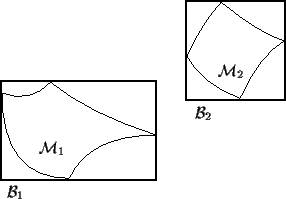
\includegraphics[scale=0.6]{img/bb1.png}
		\caption{Examplary BBs: $B_1$ is BB of $M_1$, $B_2$ is BB of $M_2$ (source: \url{http://www.idav.ucdavis.edu/education/GraphicsNotes/Bounding-Box/Bounding-Box.html})}
		\label{fig5_bbExample}
	\end{center}
\end{figure}

In the case of (1), an ROI's BB is copied pixel by pixel into a new image. The resizing (scaling the output image up or down to the provided pixel values) in the case of (2) makes preprocessing of the BB necessary. This has 2 reasons:
\begin{itemize}
	\item If the aspect ration of the provided width and height is different than the one of the BB, the resulting image will be distorted.
	\item When scaling images down, interpolation can be used, to reduce the information loss of the image\cite{Thevanez00}. This is partially possible when scaling images up as well, e.g. via fractal interpolation, but a non trivial task\cite{Guerdri16}.
\end{itemize}

Therefore, the size of the BB will be adjusted to match the aspect ratio of the provided width and height. If the resulting BB is bigger then the provided width and height, the image will be scaled down and interpolated. If the BB is smaller, it will be scaled up instead of the image. This leads to a bigger area inside the BB that is not part of the ROI, but a pixel ratio of 1:1 between original and extracted image, resulting in no distortion or loss of quality.

Case (3) approximates a ROI by tessellating\footnote{
	\emph{Tessellation} describes the tiling of a plane using one or more geometric shapes with no overlaps or gaps\cite{Clifford09}.
} it into tiles of the provided width and height (see fig. \ref{fig5_tesExample} for an example). Every tile inside the region's enclosing path (or touched by it) is targeted by the extraction. Each tile is extracted into an individual image.

\begin{figure}[H]
	\begin{center}
		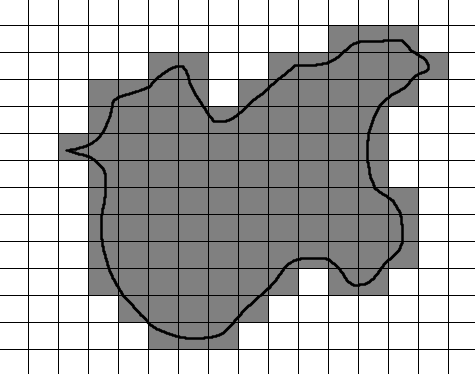
\includegraphics[scale=0.5]{img/tessellation.png}
		\caption{Example of an ROI approximated via tessellation (gray tiles belong to the ROI)}
		\label{fig5_tesExample}
	\end{center}
\end{figure}

Cases (1) - (3) can be combined with (4) to convert the extracted ROI images into grayscale images.

A region contains additional information besides the label that can be utilized, especially the level of magnification\footnote{
	Compare subsection \ref{sec4_region}
}. As Doyle has shown in \cite{Doyle10}, the level of magnification an annotation was made in is an important factor. This is due to the fact that manual annotations made in lower magnifications do not have the granularity needed for higher ones, which results in numerous false positives and negatives and therefore distorts the ground truth\cite{Janowczyk16}. A region's zoom attribute informs at what level of magnification a region was drawn in, thus helping to assess the described issue.

To utilize the additional metadata, each extracted region will also have a corresponding metadata file. This metadata contains:
\begin{itemize}
	\item the name of the extracted image file (case (1) and (2)), or a list of all image tiles which belong to the ROI (case (3))
	\item the region's label
	\item the level of magnification
	\item the region's context
\end{itemize}

Section \ref{sec5_objective} additionally stated the objective of keeping up correspondence between an ROI and its associated label. To achieve this, an extracted image will be saved in a directory of the same name as its corresponding label. This way, all ROIs of a specific label can be collected in one location. Additionally, the corresponding metadata file will contain an association between image file and label name.


\section{Implementation}
\label{sec5_impl}
The TS is implemented as a python script called \textbf{\emph{TessellationService.py}}\footnote{
	See its GitHub repository for more information: \url{https://github.com/SasNaw/TessellationService}.
}. As stated in sections \ref{sec5_objective} and \ref{sec5_method}, its purpose is to extract annotated ROIs from a WSI. This is done with the help of the following frameworks and libraries: \emph{OpenSlide}, \emph{NumPy}, \emph{Pillow} and \emph{OpenCV} (Open Source Computer Vision Library)\nmc{OpenCV}{Open Source Computer Vision Library}.

\emph{OpenSlide} was used to access and read a provided WSI\footnote {
	Compare subsection \ref{sec4_asvFrameworks} - OpenSlide
}.

NumPy is a python library for efficient scientific computing, especially regarding operations involving multi-dimensional array objects\cite{Walt11}. Since a lot of image operations are based on the use of matrices, this library was used to increase efficiency.

OpenCV is an open source computer vision and machine learning software library. It was built to provide a common infrastructure for computer vision applications. It offers numerous functions regarding image processing and machine learning, with a strong focus on real-time computing and efficiency\cite{Bradski08}. Its main purpose in the TS is to create a reference image for the tessellation function\footnote{
	See subsection \ref{sec5_tessellation}
}

Pillow is an imaging library, which offers methods to read from and write to images. It was used for reading, writing, scaling and converting the extracted images.

A detailed documentation of the TS' functions can be found in appendix \ref{secC}.

\subsection{Execution}
\label{sec5_exec}
The TS can be called over the python interpreter:

\begin{lstlisting}
	$ python TessellationService [input] [dictionary] [params]
\end{lstlisting}

The arguments [input] and [dictionary] are mandatory. The files which are supposed to be targeted by the extraction process are handed to the TS via the \emph{[input]} argument. This can be a list of WSIs, DZIs and directories. If a directory is handed to the TS, all subdirectories (except a DZI's \emph{"{\textunderscore}files"} directory) will be searched as well.

As mentioned in chapter \ref{sec4_as}, multiple dictionaries can be used for annotation. Since every WSI has an individual save file for each dictionary (compare subsection \ref{sec4_setup}), it is necessary to provide the dictionary targeted for extraction via the [dictionary] parameter. Each input file must have its associated save file in the same directory.



As mentioned in section \ref{sec5_method}, it might be necessary to create different output images for different purposes. Therefore, the TS has a list of optional parameters to manipulate the created output in order to be applicable to a wider variety of cases (see tab. \ref{tab5_tsParams}). Those parameters are optional. 

\begin{table}[H]
	\begin{center}
		\begin{tabular}{| p{3cm} | p{5cm} | p{3cm} |}
			\hline
			\textbf{name} & \textbf{description} & \textbf{default}\\ \hline
			-h, --help & show help & - \\ \hline
			-f, --force-overwrite & flag to overwrite images with the same name (if not supplied, a number will be added to the image name) & false \\ \hline
			-g, --grayscale & flag to convert images to grayscale images before saving them & false \\ \hline
			-i, --interpolation & choose interpolation method: nearest neighbor, bilinear, bicubic, lanczos  & nearest neighbor interpolation \\ \hline
			-o, --output [directory] & choose output directory (if not provided, the TS will save all extracted images in its current working directory) & - \\ \hline
			-r, --resize [width] [height] & resize all output images to the provided [width] and [height] in pixel & - \\ \hline
			-s, --show-tessellated & flag to create window and show stitched image resulting from the tessellation process (only for debugging purposes, see \emph{"-t"}) & false\\ \hline
			-t, --tessellate [width] [height] & tessellate regions into tiles of the provided [width] and [height] in pixels & - \\ \hline
		\end{tabular}
		\caption{Optional parameters for the TS}
		\label{tab5_tsParams}
	\end{center}
\end{table}


\subsection{Extraction process}
\label{sec5_extractionProcess}
The TS receives a list of files and folders to extract regions from and iterates over each entry. If the entry is a directory, each contained element will be checked for its type. If it is a WSI/DZI file, the extraction is started right away. Once the extraction is finished, the next element is examined. If the entry is a directory, each contained element is subject to the same evaluation. WSI/DZI files are extracted, while subdirectories are recursively traversed until the end of the directory tree. Each element found in this process that qualifies for region extraction is extracted. Fig. \ref{fig5_tsRunUml} visualizes the described process in an activity diagram.

\begin{figure}[H]
	\begin{center}
		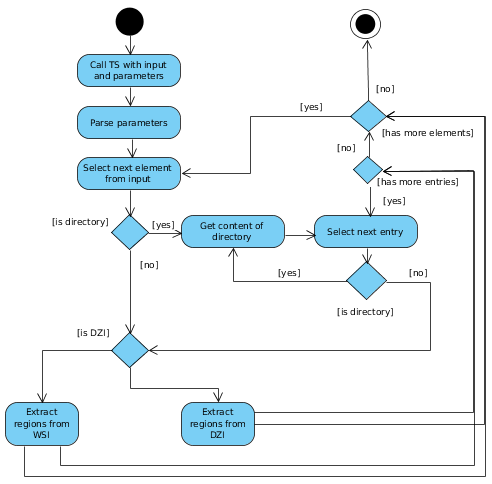
\includegraphics[scale=0.6]{img/ts_run.png}
		\caption{Activity diagram of TS' extraction procedure}
		\label{fig5_tsRunUml}
	\end{center}
\end{figure}

OpenSlide is used to read a provided WSI. Since OpenSlide can not open a native DZI, but only wrap an OpenSlide object into a DZG\footnote{
	Compare subsection \ref{sec4_openslide}
}, a different approach had to be chosen to access a provided DZI.

Both approaches share the following utility functions\footnote{
	See appendix \ref{secC} for documentation of the individual function's source code.
}:

\begin{itemize}
	\item \texttt{read{\textunderscore}json(path)} tries to read the JSON file at the provided path. If successful, it returns a list with the regions parsed from the file. If the file was not found or corrupt, a message will be printed on the terminal, informing the user about the exception.
	
	\item \texttt{save{\textunderscore}image(image, region, slide{\textunderscore}name, *tiles)} generates an appropriate name from the region information and the slide{\textunderscore}name for the image and metadata file. The name differs between tessellated and non-tessellated output (see tab. \ref{tab5_outputNames}).
	
	If -r is provided, the image will be resized to the supplied height and width, with the interpolation method provided via -i (default: nearest neighbor interpolation). If -g is specified, the image will be converted to grayscale with the luma transform defined in the ITU-R 601-2 standard\cite{ITUR94} (see eq. \ref{eq:luma}).
	\begin{equation}\label{eq:luma}
		L = R * 299/1000 + G * 587/1000 + B * 114/1000
	\end{equation}
	
	Eq. \ref{eq:luma} averages out the RGB values of every pixel under consideration of how a human eye perceives colors.
	
	If -o was provided, the processed image will be saved in the supplied location inside a directory with the name of the extracted region's label.
	
	\item \texttt{save{\textunderscore}metadata(name, region, *tiles)} writes the corresponding metadata to an extracted image into a file (see tab. \ref{tab5_outputNames} for the file name pattern). The metadata is a JSON map and contains the values listed in tab. \ref{tab5_metadataJson}. When the TS is run with -t, the \emph{"image"} key is replaced by \emph{"tiles"}, which contains a JSON list with the names of all tiles belonging to the extracted image (each individual image name is according to the pattern in tab. \ref{tab5_outputNames}).
	
	\begin{table}[H]
		\begin{center}
			\begin{tabular}{| l | p{6cm} | l |}
				\hline
				\textbf{key} & \textbf{value} & \textbf{type}\\ \hline
				context & the image region's context & JSON list\\ \hline
				image & name of the extracted image file (compare tab. \ref{tab5_outputNames}) & string \\ \hline
				label & the region's label & string\\ \hline
				zoom & the region's zoom & float\\ \hline
			\end{tabular}
			\caption{File name patterns of generated output}
			\label{tab5_metadataJson}
		\end{center}
	\end{table}
	
	\item \texttt{get{\textunderscore}bounding{\textunderscore}box(region)} iterates over every segment of a region's path and builds the BB by collecting the minimal and maximal values for x and y (compare fig. \ref{fig5_bbExample}).
	
	\item \texttt{resize{\textunderscore}bounding{\textunderscore}box(bounding{\textunderscore}box)} is used to adjust a region's BB to a different aspect ratio. This is to avoid image distortion when the -r parameter specifies a different image ratio than the BB's inherent one (see fig. \ref{fig5_resizeBBexample} for an example).
	
	\begin{figure}[H]	
		\begin{center}
			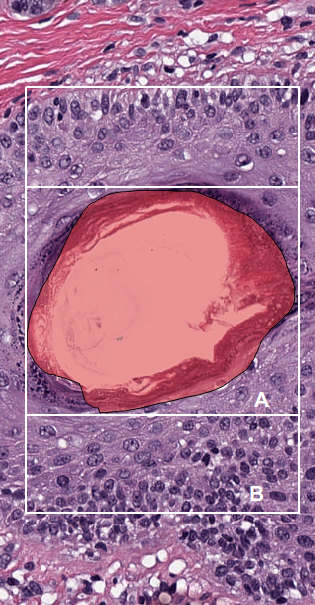
\includegraphics[scale=0.3]{img/bbResizeExample.png}
			\caption{Example for adjusted BB (A - original BB with aspect ratio of $\sim$1:1, B - adjusted BB to aspect ratio of $\sim$1:2)}
			\label{fig5_resizeBBexample}
		\end{center}
	\end{figure}
	
	\item \texttt{scale{\textunderscore}bounding{\textunderscore}box(bounding{\textunderscore}box, scale)} scales a BB by a provided scale. This is to avoid image distortions due to scaling images up (compare section \ref{sec5_method}). While \texttt{get{\textunderscore}bounding{\textunderscore}box(region)} changes the aspect ratio of a BB, \texttt{scale{\textunderscore}bounding{\textunderscore}box(bounding{\textunderscore}box, scale)} keeps the aspect ratio and changes the BB as a whole instead.
\end{itemize}

\begin{table}[H]
	\begin{center}
		\begin{tabular}{| p{3cm} |p{4cm} | p{4cm} |}
			\hline
			\textbf{name} & \textbf{image file} & \textbf{metadata file}\\ \hline
			\textbf{-t not provided} & [slide{\textunderscore}name]{\textunderscore}[region.uid].{\newline}jpeg & [slide{\textunderscore}name]{\textunderscore}[region.uid].{\newline}metadata.json \\ \hline
			\textbf{-t provided}  & [slide{\textunderscore}name]{\textunderscore}[region.uid]\newline([row]{\textunderscore}[column]).jpeg & [slide{\textunderscore}name]{\textunderscore}[region.uid].{\newline}metadata.tessellated.json \\ \hline
		\end{tabular}
		\caption{File name patterns of generated output}
		\label{tab5_outputNames}
	\end{center}
\end{table}


\subsection{Extraction without Tessellation}
\label{sec5_extraction}
As mentioned above, the implementation of the conversion differs for WSI and DZI due to the role of OpenSlide in the extraction of WSIs. The following two sections describe the extraction process for both cases.

\subsubsection{WSI}
The WSI extraction process is done in the \texttt{wsi(file)} function\footnote{
	See appendix \ref{secC} for a function documentation.
}. It opens the provided file via OpenSlide, builds a name from its path and parses the regions of the WSI via \texttt{read{\textunderscore}json(path)}. The function iterates over every parsed region to extract it. The extraction process is visualized in fig. \ref{fig5_tsWsiUml}. 

\begin{figure}[H]
	\begin{center}
		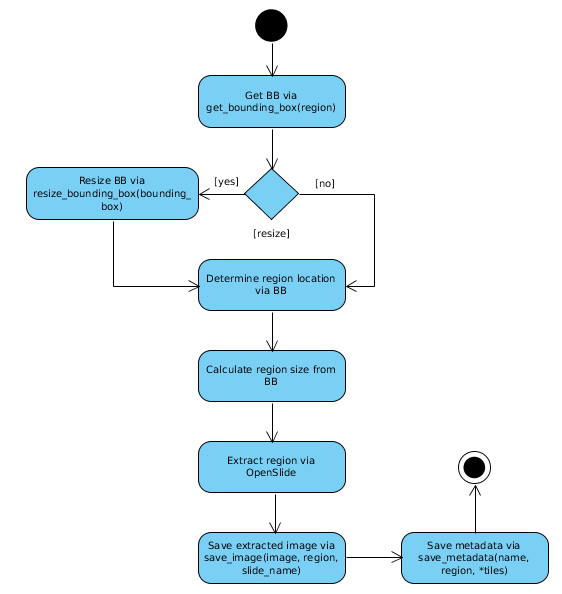
\includegraphics[scale=0.45]{img/ts_wsi_uml.png}
		\caption{Activity diagram of TS' WSI extraction (without tessellation)}
		\label{fig5_tsWsiUml}
	\end{center}
\end{figure}

As shown in fig. \ref{fig5_tsWsiUml}, calculating the BB is the first step. To do so, the \texttt{get{\textunderscore}bounding{\textunderscore}box(region)} function is used, which returns a python dictionary with the minimum and maximum values of x and y in the associated region's path. If -r was provided, the BB's size will be adjusted to fit the supplied image ratio.

Next, the location of the region is determined. This is done by taking the minimum value for x and y from the BB and declaring it as upper, left corner of the region. The size is calculated by subtracting the minimum from the maximum value for x and y respectively (see eq. \ref{eq:sizeX} and \ref{eq:sizey}).

\begin{equation}\label{eq:sizeX}
size_x = BB_{max(x)} - BB_{min(x)}
\end{equation}
\begin{equation}\label{eq:sizey}
size_y = BB_{max(y)} - BB_{min(y)}
\end{equation}

OpenSlide's \texttt{readRegion(location, level, size)} function is used to retrieve the region in a separate image from the original baseline image. This extracted image is then written into a file, together with its associated region's metadata.

\subsubsection{DZI}
Since it is not possible to open a DZI with OpenSlide, the extraction process for DZI differs from the one for WSI. It is implemented in the \texttt{dzi(file)} function\footnote{
	See appendix \ref{secC} for a function documentation.
}, which starts and manages the extraction process. Since an image must be stitched together manually, the information about tile size and image dimensions must be parsed from the DZI metadata file, as well as the level containing the baseline image (since DZI uses n instead of 0 for the level with the highest resolution). Once the information is parsed, a file name is created from the file path and the corresponding regions are parsed from the associated JSON file. Fig. \ref{fig5_tsDziUml} visualizes the extraction process and its individual steps, which are executed for each region.

\begin{figure}[!h]
	\begin{center}
		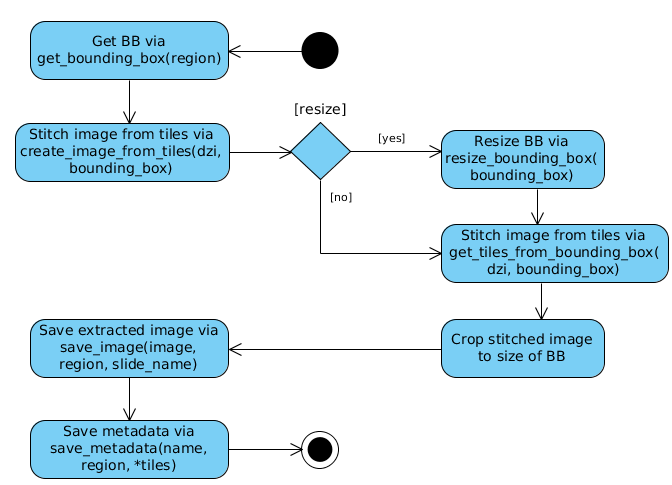
\includegraphics[scale=0.45]{img/ts_dzi_uml.png}
		\caption{Activity diagram of TS' DZI extraction (without tessellation)}
		\label{fig5_tsDziUml}
	\end{center}
\end{figure}

The BB is created via the \texttt{get{\textunderscore}bounding{\textunderscore}box(region)} function. Once the BB is created, the stitching process of the area covered by the baseline image begins. This is realized in the \texttt{create{\textunderscore}image{\textunderscore}from{\textunderscore}tiles(dzi, bounding{\textunderscore}box)} function. It first checks, if the -r parameter was provided and if so, if the aspect ratio of the BB matches the ratio of the supplied height and width. If necessary, the BB is adjusted via \texttt{resize{\textunderscore}bounding{\textunderscore}box(bounding{\textunderscore}box)}.
 
The first step in stitching the baseline image area together, is determining the size of the BB (see eq. \ref{eq:sizeX} and \ref{eq:sizey}). To determine the needed tiles, $BB_{min(x)}$, $BB_{min(y)}$, $BB_{max(x)}$ and $BB_{max(y)}$ are divided by the DZI's tile size, resulting in $BB_{min(x)}^t$, $BB_{min(y)}^t$, $BB_{max(x)}^t$ and $BB_{max(y)}^t$. Those values are then iterated from the pair $(BB_{min(x)}^t, BB_{min(y)}^t)$ to $(BB_{max(x)}^t, BB_{max(y)}^t)$. Each of the resulting pairs $(BB_x^t, BB_y^t)$ refers to a tile from the baseline image. The baseline image area is stitched together by iterating over all pairs $(BB_x^t, BB_y^t)$ and stitching the corresponding tiles together. This is implemented in the \texttt{get{\textunderscore}image{\textunderscore}from{\textunderscore}bounding{\textunderscore}box(dzi, bounding{\textunderscore}box)} function. The stitched image is then cropped to fit the size and position of the BB and saved together with its corresponding metadata file (via \texttt{save{\textunderscore}file(image, region, slide{\textunderscore}name)} and \texttt{save{\textunderscore}metadata(name, region, *tiles)}).


\subsection{Extraction with Tessellation}
\label{sec5_tessellation}

If a region is extracted with the -t parameter (compare tab. \ref{tab5_tsParams}), it will be tessellated into multiple image tiles of provided width and height (compare \ref{sec5_method}(3) and fig. \ref{fig5_tesExample}). As in subsection \ref{sec5_extraction}, the main difference between the processing of a WSI and a DZI is the need to parse the DZI's associated metadata and stitch an area of the baseline image. With that exception, the tessellated extraction works identical in both cases.

The baseline image is tessellated into $m$*$n$ virtual tiles (see eq. \ref{eq:m} and \ref{eq:n}). All virtual tiles containing parts of the region's path are saved in a list $L^{path}$.
\begin{equation}\label{eq:m}
	m = \text{baseline image height} / \text{tile height}
\end{equation}
\begin{equation}\label{eq:n}
	n = \text{baseline image width} / \text{tile width}
\end{equation}

The virtual tiles are needed to create and work with the \emph{reference image} (RI\nmc{RI}{Reference Image}). The RI is a central component of the tessellated extraction process. It is a binary image, which is $m$ pixels high and $n$ pixels wide. Each pixel represents a virtual tile of the baseline image. If a pixel is white, the corresponding virtual tile is part of the region to extract.The RI is a matrix representation of which tile is needed from the baseline image (see fig. \ref{fig5_riExample}).

\begin{figure}[!h]
	\begin{center}
		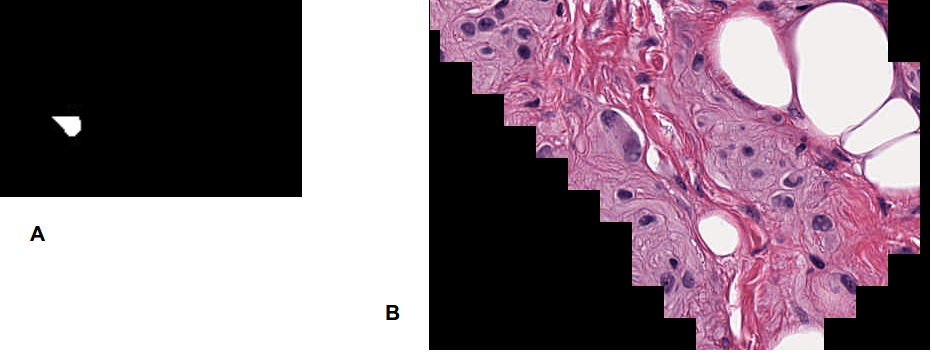
\includegraphics[scale=0.35]{img/RI_example.png}
		\caption{Example of RI (A) and resulting image tiles (B, stitched) with a tile size of 32x32 pixel (example was created using CMU-1.svs from Aperio, see appendix \ref{secA})}
		\label{fig5_riExample}
	\end{center}
\end{figure}

When created, the RI has only black pixels. To color the pixels associated with the ROI white,  OpenCV's \texttt{drawContours(image, contours, color, fill)} function is used. Since the correspondence of pixels and tiles is bidirectional, $L^{path}$ can be used to describe the contour. The drawn contour is then filled white.

The last step is to iterate each pixel of the RI. For every white pixel found, the corresponding tile is extracted from the baseline image and saved into an individual image file (compare tab. \ref{tab5_outputNames} for the naming convention).


\section{Test}
\label{sec5_test}
The TS was run on multiple WSIs from the test data set (see appendix \ref{secA}). The test case presented in the following subsections is based on \emph{CMU-1.svs} of the Aperio test set\footnote{
	Obtainable at \url{http://openslide.cs.cmu.edu/download/openslide-testdata/Aperio/}
} The JSON file used for the test can be found in the git repository of the TS, in the \emph{"test"} branch\footnote{
	See \url{https://github.com/SasNaw/TessellationService/tree/test}
}. The annotations were made using the \emph{example.json} dictionary.


\subsection{Setup}
\label{sec5_testSetup}
The WSI CMU-1.svs, its corresponding JSON file CMU-1.svs{\textunderscore}example.json and TessellationService.py were placed in the same directory. To ensure that all parameters work correctly, the TS was provided with different parameters in multiple test cases (see tab. \ref{tab5_tests}).

The provided JSON file has 3 saved annotations (see fig. \ref{fig5_sample}), to test the behavior of small (BB of 39x41 pixel, see fig. \ref{fig5_sample:3}), medium (BB of 346x288 pixel, see fig. \ref{fig5_sample:1}) and large sized images (BB of 6085x1540 pixel, see fig. \ref{fig5_sample:2}). All test cases were executed with those 3 regions.

\begin{table}[H]
	\begin{center}
		\begin{tabular}{| p{1.5cm} | p{3cm} |  p{5.5cm} |}
			\hline
			\textbf{test \#} & \textbf{parameters} & \textbf{description}\\ \hline
			1 & -o noparams & no parameters provided, except -o \\ \hline
			2 & -o square -r 256 256 & resize every image to 256x256 pixels (aspect ratio of 1:1)\\ \hline
			3 & -o rectangle -r 256 128 & resize every image to 256x128 pixels (aspect ratio of 2:1) \\ \hline
			4 & -o tessellate -t 32 32 & tessellation of ROIs with 32x32 pixel sized tiles \\ \hline
			5 & -o grayscale -r 256 256 -g & resize every image to 256x256 pixels and turn them to grayscale\\ \hline
		\end{tabular}
		\caption{Test cases for the TS}
		\label{tab5_tests}
	\end{center}
\end{table}

\begin{figure}[!h]
	\begin{subfigure}{.6\textwidth}
		\centering
		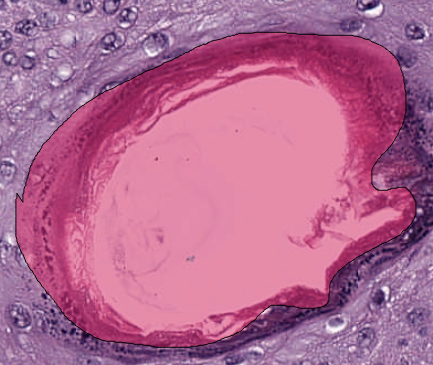
\includegraphics[width=.8\linewidth]{img/ts_test/region1.png}
		\caption{test region A (BB = 364x288 pixel)}
		\label{fig5_sample:1}
	\end{subfigure}%
	\begin{subfigure}{.2\textwidth}
		\centering
		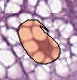
\includegraphics[width=.8\linewidth]{img/ts_test/region3.png}
		\caption{test region B (BB = 39x41 pixel)}
		\label{fig5_sample:3}
	\end{subfigure}
	\begin{subfigure}{1\textwidth}
		\centering
		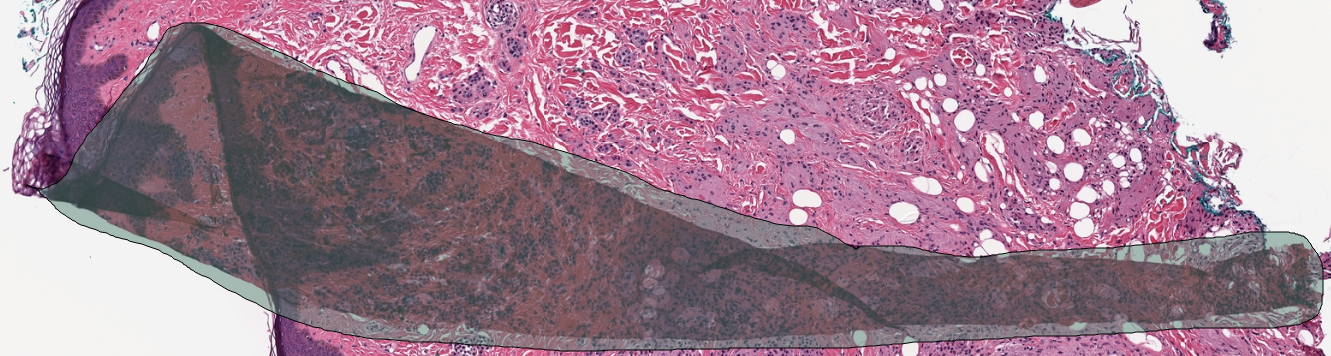
\includegraphics[width=1\linewidth]{img/ts_test/region2.png}
		\caption{test region C (BB = 6085x1540 pixel)}
		\label{fig5_sample:2}
	\end{subfigure}
	\caption{Test case \emph{Aperio - CMU-1.svs}}
	\label{fig5_sample}
\end{figure}
\clearpage

\subsection{Result}

Fig. \ref{fig5_result1} - \ref{fig5_result3} show the results of the test cases described in tab. \ref{tab5_tests}. Tab. \ref{tab5_results} shows how the results correspond to the tests.

\begin{table}[H]
	\begin{center}
		\begin{tabular}{| l | l |}
			\hline
			\textbf{test \#} & \textbf{figures}\\ \hline
			1 & \ref{subfig5:a1}, \ref{subfig5:b1}, \ref{subfig5:c1}\\ \hline
			2 & \ref{subfig5:a2}, \ref{subfig5:b2}, \ref{subfig5:c2}\\ \hline
			3 & \ref{subfig5:a3}, \ref{subfig5:b3}, \ref{subfig5:c3}\\ \hline
			4 & \ref{subfig5:a4}, \ref{subfig5:b4}, \ref{subfig5:c4}\\ \hline
			5 & \ref{subfig5:a5}, \ref{subfig5:b5}, \ref{subfig5:c5}\\ \hline
		\end{tabular}
		\caption{Test-result correspondence}
		\label{tab5_results}
	\end{center}
\end{table}

The extraction without parameters was successful in every case (see \ref{subfig5:a1}, \ref{subfig5:b1}, \ref{subfig5:c1}).

The BBs were successfully adjusted and the images scaled to the provided size (\ref{subfig5:a1}, \ref{subfig5:b2}, \ref{subfig5:c2} and \ref{subfig5:a3}, \ref{subfig5:b3}, \ref{subfig5:c3}).

The tessellation of ROIs was successful for all provided regions (\ref{subfig5:a4}, \ref{subfig5:b4}, \ref{subfig5:c4}), as was the conversion to grayscale (\ref{subfig5:a5}, \ref{subfig5:b5}, \ref{subfig5:c5}).

\begin{figure}[H]
	\begin{subfigure}{.5\textwidth}
		\centering
		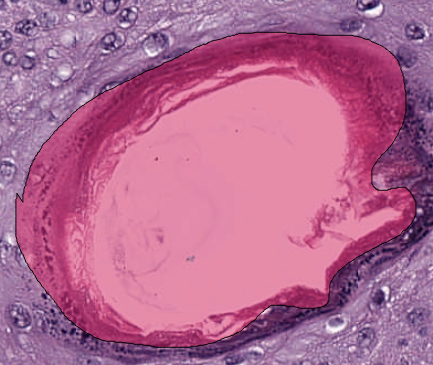
\includegraphics[width=.8\linewidth]{img/ts_test/region1.png}
		\caption{Test region A in the ASV}
	\end{subfigure}
	\begin{subfigure}{.5\textwidth}
		\centering
		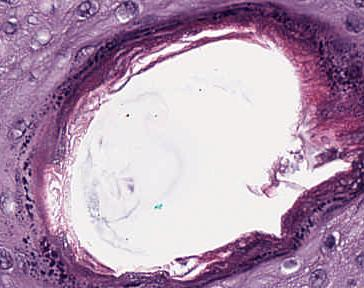
\includegraphics[width=.8\linewidth]{img/ts_test/1_orig.jpeg}
		\caption{Extracted without parameters}
		\label{subfig5:a1}
	\end{subfigure}
	\begin{subfigure}{.5\textwidth}
		\centering
		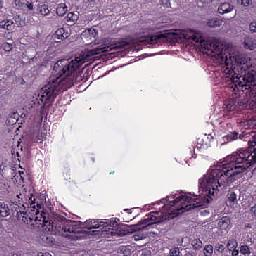
\includegraphics[width=.8\linewidth]{img/ts_test/1_r256.jpeg}
		\caption{Extracted and resized to 256x256 pixel}
		\label{subfig5:a2}
	\end{subfigure}
	\begin{subfigure}{.5\textwidth}
		\centering
		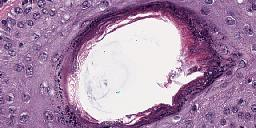
\includegraphics[width=.8\linewidth]{img/ts_test/1_r128.jpeg}
		\caption{Extracted and resized to 256x128 pixel}
		\label{subfig5:a3}
	\end{subfigure}
	\begin{subfigure}{.5\textwidth}
		\centering
		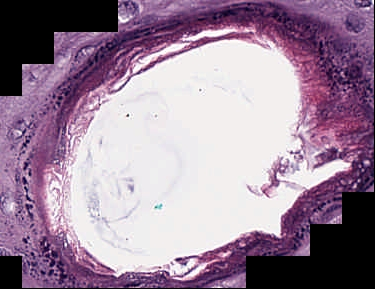
\includegraphics[width=.8\linewidth]{img/ts_test/1_stitched.jpeg}
		\caption{Tessellated into 32x32 pixel sized tiles}
		\label{subfig5:a4}
	\end{subfigure}
	\begin{subfigure}{.5\textwidth}
		\centering
		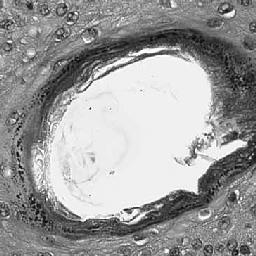
\includegraphics[width=.8\linewidth]{img/ts_test/1_g.jpeg}
		\caption{Extracted, resized and converted to grayscale}
		\label{subfig5:a5}
	\end{subfigure}
	\caption{Results for test region A}
	\label{fig5_result1}
\end{figure}

\begin{figure}[H]
	\begin{subfigure}{.5\textwidth}
		\centering
		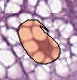
\includegraphics{img/ts_test/region3.png}
		\caption{Test region B in ASV}
	\end{subfigure}
	\begin{subfigure}{.5\textwidth}
		\centering
		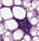
\includegraphics{img/ts_test/3_orig.jpeg}
		\caption{Extracted without parameters}
		\label{subfig5:b1}
	\end{subfigure}
	\begin{subfigure}{.5\textwidth}
		\centering
		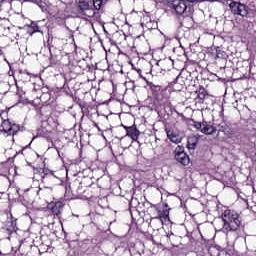
\includegraphics[width=.8\linewidth]{img/ts_test/3_r256.jpeg}
		\caption{Extracted and resized to 256x256 pixel}
		\label{subfig5:b2}
	\end{subfigure}
	\begin{subfigure}{.5\textwidth}
		\centering
		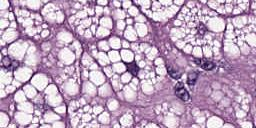
\includegraphics[width=.8\linewidth]{img/ts_test/3_r128.jpeg}
		\caption{Extracted and resized to 256x128 pixel}
		\label{subfig5:b3}
	\end{subfigure}
	\begin{subfigure}{.5\textwidth}
		\centering
		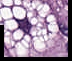
\includegraphics{img/ts_test/3_stitched.jpeg}
		\caption{Tessellated into 32x32 pixel sized tiles}
		\label{subfig5:b4}
	\end{subfigure}
	\begin{subfigure}{.5\textwidth}
		\centering
		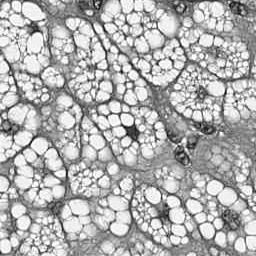
\includegraphics[width=.8\linewidth]{img/ts_test/3_g.jpeg}
		\caption{Extracted, resized and converted to grayscale}
		\label{subfig5:b5}
	\end{subfigure}
	\caption{Results for test region B}
	\label{fig5_result2}
\end{figure}

\begin{figure}[H]
	\begin{subfigure}{1.\textwidth}
		\centering
		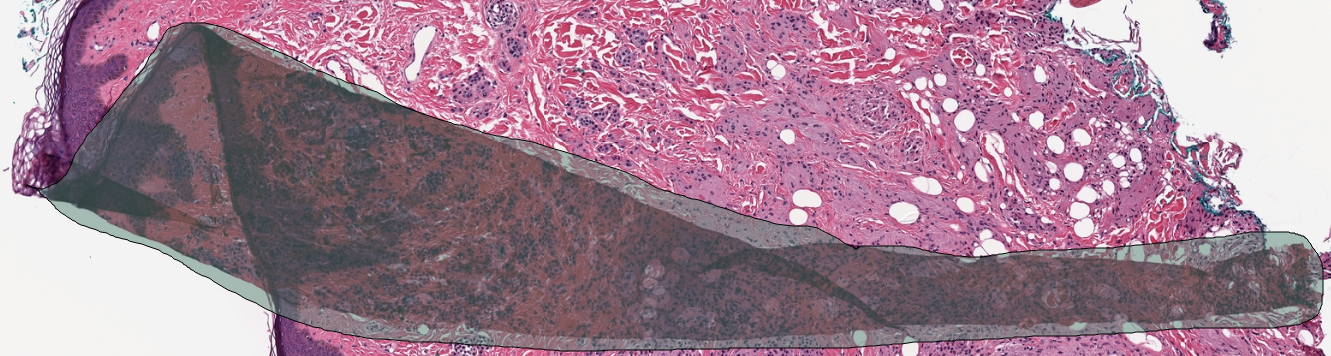
\includegraphics[width=1.\linewidth]{img/ts_test/region2.png}
		\caption{Test region C in ASV}
	\end{subfigure}
	\begin{subfigure}{1.\textwidth}
		\centering
		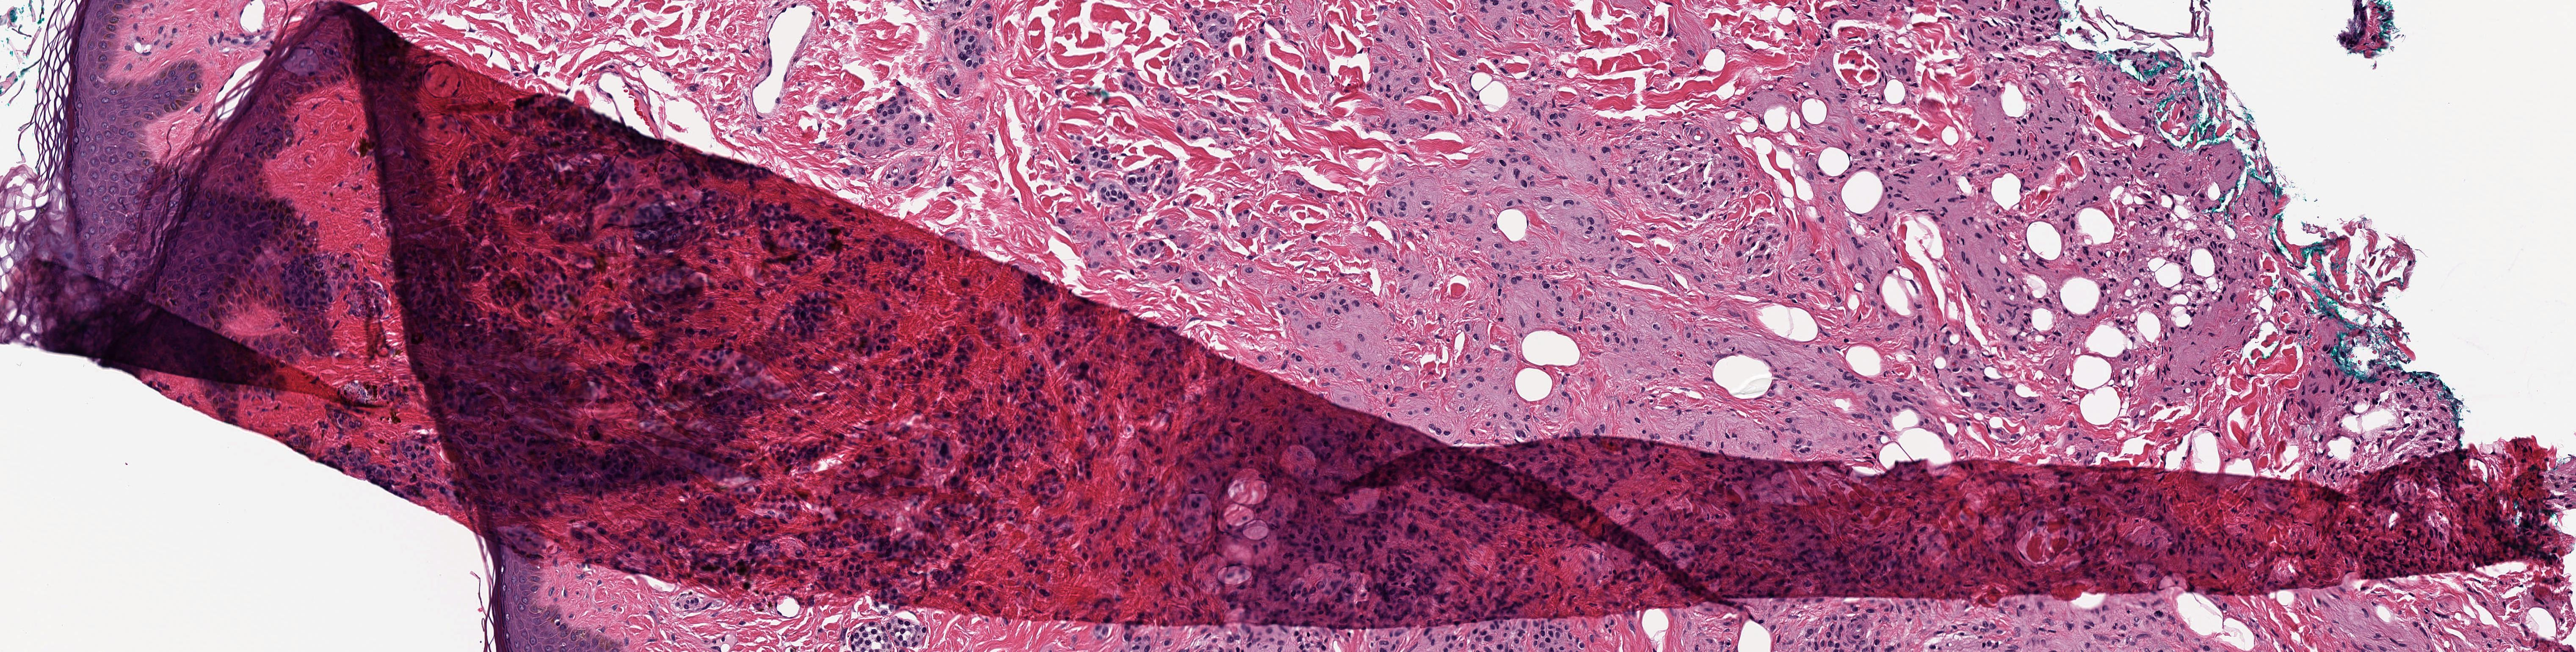
\includegraphics[width=1.\linewidth]{img/ts_test/2_orig.jpeg}
		\caption{Extracted without parameters}
		\label{subfig5:c1}
	\end{subfigure}
	\begin{subfigure}{.5\textwidth}
		\centering
		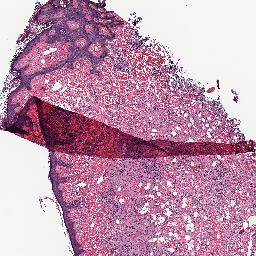
\includegraphics[width=.8\linewidth]{img/ts_test/2_r256.jpeg}
		\caption{Extracted and resized to 256x256 pixel}
		\label{subfig5:c2}
	\end{subfigure}
	\begin{subfigure}{.5\textwidth}
		\centering
		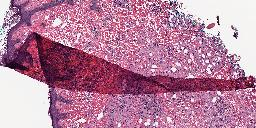
\includegraphics[width=.8\linewidth]{img/ts_test/2_r128.jpeg}
		\caption{Extracted and resized to 256x128 pixel}
		\label{subfig5:c3}
	\end{subfigure}
	\begin{subfigure}{.5\textwidth}
		\centering
		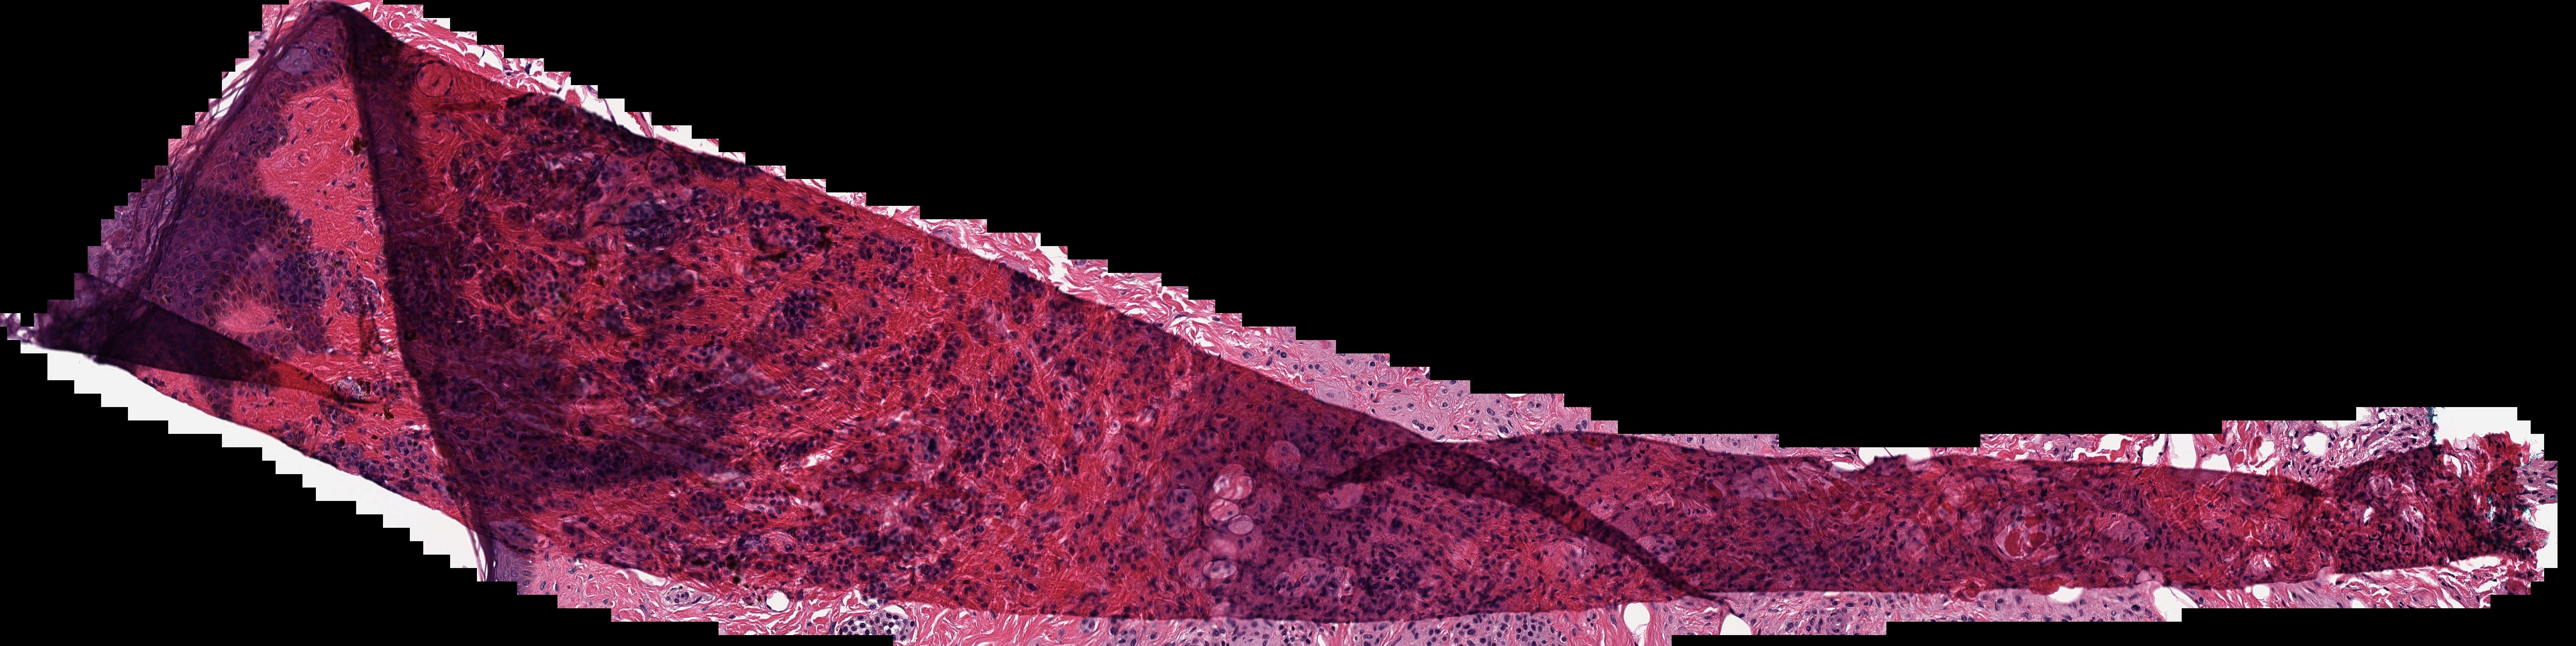
\includegraphics[width=1.\linewidth]{img/ts_test/2_stitched.jpeg}
		\caption{Tessellated into 32x32 pixel sited tiles}
		\label{subfig5:c4}
	\end{subfigure}
	\begin{subfigure}{.5\textwidth}
		\centering
		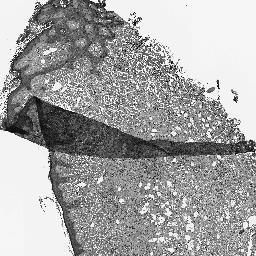
\includegraphics[width=.8\linewidth]{img/ts_test/2_g.jpeg}
		\caption{Extracted, resized and converted to grayscale}
		\label{subfig5:c5}
	\end{subfigure}
	\caption{Results for test region C}
	\label{fig5_result3}
\end{figure}
